
%(BEGIN_QUESTION)
% Copyright 2007, Tony R. Kuphaldt, released under the Creative Commons Attribution License (v 1.0)
% This means you may do almost anything with this work of mine, so long as you give me proper credit

Examine this water filter control system, then answer the following questions:

$$\includegraphics[width=15.5cm]{i01812x01.eps}$$

\begin{itemize}
\item{} Identify all primary and secondary (cascaded) loops.
\item{} The necessary control actions (direct/reverse) for each controller, assuming direct-acting transmitters and signal-to-open control valves.
\item{} What will happen to the filter water level if the influent supply suddenly shuts off?
\item{} What will happen to the clearwell reservoir water level if the influent supply suddenly shuts off?
\end{itemize}

\vskip 20pt \vbox{\hrule \hbox{\strut \vrule{} {\bf Suggestions for Socratic discussion} \vrule} \hrule}

\begin{itemize}
\item{} A useful analytical technique for any complex control system is to annotate the diagram with ``+'' and ``$-$'' symbols at the instrument bubble inputs, designating ``noninverting'' and ``inverting'' characteristics, respectively.  Show how this helps you track of all directions of action, making it easier to figure out how the control system responds to changes.
\item{} For those students who have studied level measurement, what kind of transmitters are being used here and how do they function?
\item{} For those students who have studied flow measurement, what kind of transmitters are being used here and how do they function?
\item{} For those who have studied PID tuning, what PID tuning parameters (qualitative) would you recommend for each controller in this system?
\item{} Explain what will happen in this system if the influent water pressure increases?
\item{} Explain what will happen in this system if the influent water pressure decreases?
\item{} Explain what will happen in this system if the effluent water demand (flow) increases?
\item{} Explain what will happen in this system if the effluent water demand (flow) decreases?
\item{} Explain what will happen in this system if the influent flow transmitter fails with a low signal.
\item{} Explain what will happen in this system if the influent flow transmitter fails with a high signal.
\item{} Explain what will happen in this system if the filter level transmitter fails with a low signal.
\item{} Explain what will happen in this system if the filter level transmitter fails with a high signal.
\item{} Explain what will happen in this system if the clearwell level transmitter fails with a low signal.
\item{} Explain what will happen in this system if the clearwell level transmitter fails with a high signal.
\end{itemize}

\underbar{file i01812}
%(END_QUESTION)





%(BEGIN_ANSWER)

\noindent
{\bf Partial answer:}

\vskip 10pt

Both flow controllers must be {\it reverse-acting}.  The filter level controller must be {\it direct-acting}, while the clearwell reservoir level controller must be {\it reverse-acting}.  In the event of a water supply failure, the clearwell will fail low (become empty).

%(END_ANSWER)





%(BEGIN_NOTES)

The flow controllers are secondary (slave) loops to the primary (master) level controllers.

\vskip 10pt

In the event of a water supply failure, the filter retains (almost) all its water.






\vskip 20pt \vbox{\hrule \hbox{\strut \vrule{} {\bf Virtual Troubleshooting} \vrule} \hrule}

This question is a good candidate for a ``Virtual Troubleshooting'' exercise.  Presenting the diagram to students, you first imagine in your own mind a particular fault in the system.  Then, you present one or more symptoms of that fault (something noticeable by an operator or other user of the system).  Students then propose various diagnostic tests to perform on this system to identify the nature and location of the fault, as though they were technicians trying to troubleshoot the problem.  Your job is to tell them what the result(s) would be for each of the proposed diagnostic tests, documenting those results where all the students can see.

During and after the exercise, it is good to ask students follow-up questions such as:

\begin{itemize}
\item{} What does the result of the last diagnostic test tell you about the fault?
\item{} Suppose the results of the last diagnostic test were different.  What then would that result tell you about the fault?
\item{} Is the last diagnostic test the best one we could do?
\item{} What would be the ideal order of tests, to diagnose the problem in as few steps as possible?
\end{itemize}


\vfil \eject

\noindent
{\bf Summary Quiz:}

Identify the effect of the clearwell level transmitter failing with a ``high signal'' (20 mA all the time):

$$\includegraphics[width=15.5cm]{i01812x01.eps}$$

\begin{itemize}
\item{} Clearwell runs dry; filter tank holds water
\vskip 5pt 
\item{} Clearwell overflows; filter tank runs dry
\vskip 5pt 
\item{} Clearwell holds water; filter tank runs dry
\vskip 5pt 
\item{} Clearwell runs dry; filter tank runs dry
\vskip 5pt 
\item{} Clearwell holds water; filter tank overflows
\vskip 5pt 
\item{} Clearwell runs dry; filter tank overflows
\end{itemize}

%INDEX% Control, strategies: cascade
%INDEX% Process: water filter flow/level control

%(END_NOTES)


